Al termine delle due esperienze è stato possibile andare a classificare immagini biomedicali utilizzando reti neurali 
convoluzionali ed ottenere buoni risultati sia implementando e allenando la rete partendo da 0, sia utilizzando un modello
precedentemente allenato. \\
É stato visto inoltre quanto sia necessario un buon dataset come punto di partenza così come vi debba essere un equilibrio tra le dimensioni
del set di training e quello del set di testing, quelle degli iperparametri, facendo attenzione anche all'architettura della CNN scelta,
 così che non presenti troppi parametri rispetto alla complessità del problema di interesse, ma nemmeno che questi siano insufficienti.\\
La difficoltà  principale nell'andare a realizzare sistemi come questi sta proprio nel dosare nella maniera più corretta tutti questi fattori, ed è necessario 
per riuscirci compiere una quantità molto elevata di training, applicando la tecnica conosciuta come \emph{trial and error}. 

É stato visto come costruire tali modelli richieda diversi step, partendo da una corretta analisi del dataset, 
elaborare i primi risultati fino a trovare gli iperparametri ottimali in seguito a vari tentativi e procedere con il fine-tuning della rete di conseguenza,
 ampliando il dataset se necessario.
Sono state passate in rassegna le tecniche per estendere il set di training di maggior uso fino a capire che nel caso di immagini biomedicali
è bene non andare a caso nella scelta di queste e che tutto dipende da quelli che sono i pattern significativi da riconoscere.
 
É bene scegliere trasformazioni che non vadano a rivoluzionare troppo gli schemi di immagine veri e propri, dunque le trasformazioni geometriche
possono essere utili solo se fatte nella misura giusta da non portare alla creazione di esempi anatomicamente incorretti
 e ciò richiede sforzo nell'andare a ricercare quale siano le migliori. 
Andare ad aggiungere limitatamente trasfomazioni \emph{pixel-wise} nel caso del secondo dataset e delle leggere rotazioni e zoom alle immagini nel primo dataset 
sono state i modi in cui sono stati ottenuti i migliori risultati. \\
Ovviamente tutto questo funziona se il modello è ben strutturato, altrimenti questo potrebbe fare da collo di bottiglia al training.\\
Infine questa esperienza mostra come l'utilizzo delle CNN possa essere esteso a vari tipi di classificazione e che 
modelli come quelli illustrati possano essere utilizzati per altri tipi di dataset affini. É sicuramente possibile sfruttare
i training fatti alle reti neurali sui due dataset e riutilizzarne i pesi per training successivi
 per l'identificazione di altre patologie, 
ad esempio andando a fare un'ulteriore distinzione
tra polmonite virale o batterica in riferimento al modello ottenuto nella prima esperienza oppure per andare a
 riconoscere malattie neurologiche che comportano una mutazione anomala dell'encefalo (che quindi possono essere riconoosciute tramite RM), 
 come ad esempio quelle neurodegenerative (es. Alzehimer), usando il secondo sistema.
 
 É possibile infatti durante ogni training salvare il modello allenato in un file e riutilizzarlo quando si vuole.\\
 Si riportano adesso le curve \emph{ROC (Receiver Operating Characteristics)} per mostrare 
 la validità dei sistemi implementati.  
 La curva ROC~\cite{Roc} è uno schema di rappresentazione grafica che permette di valutare l’efficienza 
 di un classificatore binario. L’analisi di della curva ROC è un metodo statistico utilizzato spesso in ambito biomedico. Essa rappresenta il metodo d’elezione 
per validare un test diagnostico. 
La curva ROC viene costruita mettendo in ascissa la \emph{specificità} ($\frac{TN}{TN+FP}$) e in ordinata la \emph{sensibilità} ($\frac{TP}{TP+FN}$, corrisponde a quella che nel capitolo 5 è stata definita come \emph{recall}) per tutti i possibili valori del test diagnostico. L’area sotto la curva ROC, \emph{area
under curve (AUC)}, è una misura quantitativa della bontà del classificatore, che può assumere valori tra 0.5 e
 1.0. Se il valore della AUC è compreso tra 0,9 e 1.0 significa che il classificatore è altamente accurato e possiede alto potere discriminante.
 Tanto maggiore è l’area sotto la curva (cioè tanto
più la curva si avvicina al vertice in alto a sinistra del grafico, quanto più  somiglia ad un gradino) tanto maggiore è il potere discriminante della rete.\\



\begin{figure}[hb!]
  \begin{subfigure}{0.5\textwidth}
    \centering
    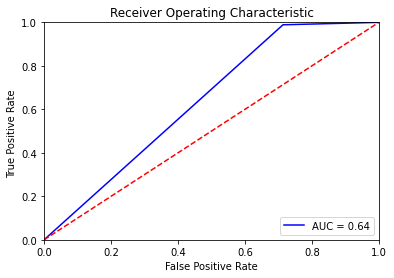
\includegraphics[width=1\textwidth]{Figures/roc-pneumonia-no-aug.png}
    %\caption{1a}
    \caption{}
    \label{fig:snap1}
  \end{subfigure}%
  \begin{subfigure}{0.5\textwidth}
    \centering
    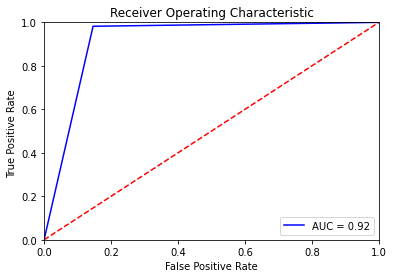
\includegraphics[width=1\textwidth]{Figures/roc-pneumonia-aug.png}
    %\caption{1a}
    \caption{}
    \label{fig:snap2}
  \end{subfigure}%
  \caption{Confronto della caratteristica ROC tra il sistema per la rilevazione della polmonite senza applicare le modifiche al set di training (a)
  e quella del sistema allenato sul set ampliato (b). Il codice di realizzazione può essere visto nel Code Listing 7.1.
  }
  \label{fig:fig}
\end{figure} 



\begin{figure}[hb!]
    \begin{subfigure}{0.5\textwidth}
      \centering
      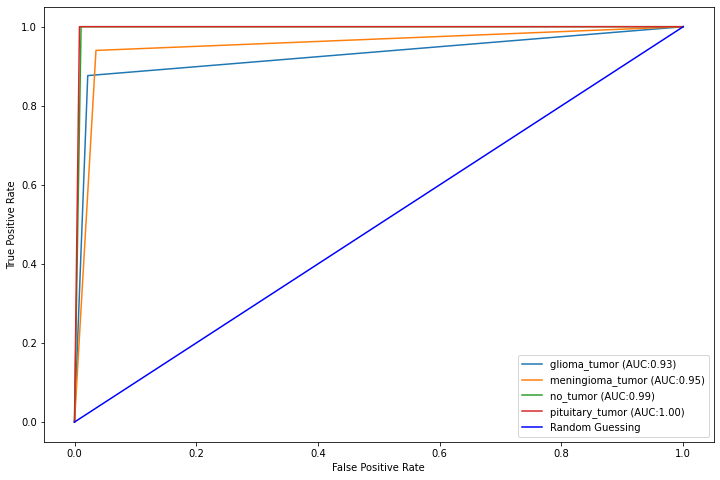
\includegraphics[width=1\textwidth]{Figures/roc-alexnet.png}
      %\caption{1a}
      \caption{}
      \label{fig:snap1}
    \end{subfigure}%
    \begin{subfigure}{0.5\textwidth}
      \centering
      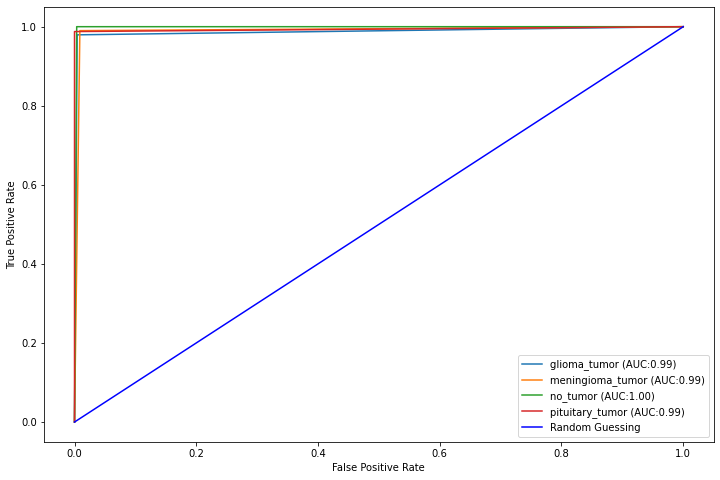
\includegraphics[width=1\textwidth]{Figures/ROC-pretrained.png}
      %\caption{1a}
      \caption{}
      \label{fig:snap2}
    \end{subfigure}%
    \caption{Confronto tra la caratteristica ROC del modello \emph{2.} con rumore gaussiano e del modello \emph{3.} per il dataset delle RM.
    (a) mostra una AUC di 0.96, (b) dello 0.99. Il codice di realizzazione può essere visto nel Code Listing 7.2.
    }
    \label{fig:fig}
\end{figure} 


 